%%%%%%%%%%%%%%%%%%%%%%%%%%%%%%%%%%%%%%%%%%%%%%%%%%%%%%%%%%%%%%%%%%%%%%%%%%
% Signal of uT1 for raising load
%%%%%%%%%%%%%%%%%%%%%%%%%%%%%%%%%%%%%%%%%%%%%%%%%%%%%%%%%%%%%%%%%%%%%%%%%%
\begin{solutionfigure}[htb]
        \centering
        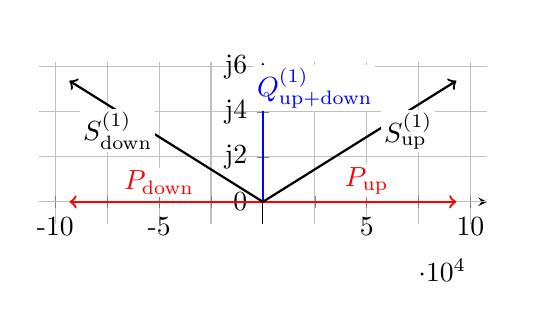
\begin{tikzpicture}
            \begin{axis}[
                % x/y range adjustment
                xmin=-10800, xmax=10800,
                ymin=-1000, ymax=6200,
                samples=500,
                axis y line=center,
                axis x line=middle,
                extra y ticks=0,
                % Label text
                xlabel={$\SI{}{\kilo\watt}$},,
                ylabel={$\SI{}{\kilo\watt}$},
                % Label adjustment
                x label style={anchor=west},
                y label style={anchor=south,yshift=0.2cm},
                width=0.6\textwidth,
                height=0.3\textwidth,
                % x-Ticks
                xtick={10000,7500,5000,2500,0,-2500,-5000,-7500,-10000},
                xticklabels={10,,5,,0,,-5,,-10},
                xticklabel style = {anchor=north},
                % y-Ticks
                ytick={6000,4000,2000,0},
                yticklabels={j6,j4,j2,},
                yticklabel style = {anchor=east},
                % Grid layout
                grid,
                %grid style={line width=.1pt, draw=gray!10},
                %major grid style={line width=.2pt,draw=gray!90},
                ]
                % Q1/2
                \draw[->,blue, solid, thick] (axis cs:0,0) -- (axis cs:0,5380);
                % Label of Qup/down
                \node[blue, fill=white, inner sep = 1pt, anchor = south] at (axis cs:2500,4000) {$Q_\mathrm{up+down}^\mathrm{(1)}$};
                %Pup
                \draw[->,red, solid, thick] (axis cs:0,0) -- (axis cs:9320,0);
                % Label of Pup
                \node[red, fill=white, inner sep = 1pt, anchor = south] at (axis cs:5000,200) {$P_\mathrm{up}$};
                %Pdown
                \draw[->,red, solid, thick] (axis cs:0,0) -- (axis cs:-9320,0);
                % Label of Pup
                \node[red, fill=white, inner sep = 1pt, anchor = south] at (axis cs:-5000,200) {$P_\mathrm{down}$};
                %Sup
                \draw[->, solid, thick] (axis cs:0,0) -- (axis cs:9320,5380);
                % Label of Pup
                \node[fill=white, inner sep = 1pt, anchor = south] at (axis cs:7000,2200) {$S_\mathrm{up}^\mathrm{(1)}$};
                %Sdown
                \draw[->, solid, thick] (axis cs:0,0) -- (axis cs:-9320,5380);
                % Label of Pup
                \node[fill=white, inner sep = 1pt, anchor = south] at (axis cs:-7000,2200) {$S_\mathrm{down}^\mathrm{(1)}$};
            \end{axis}
        \end{tikzpicture}
        \caption{Power within the complex plane}
        \label{fig:ex06_Complex_Plane_Power}
\end{solutionfigure}